%-------------------------------------------------------------------------------
\section{Results}
\label{sec:result}
%-------------------------------------------------------------------------------
\subsection{Combination of Helicity Fraction Measurements}
The template fitting method described in Section \ref{sec:templateFitting} was applied to the full 2012 dataset in the eight independent channels (electron/muon, leptonic/hadronic, one exclusive/two inclusive \bt tags) described previously. The combined measurement was obtained by extending the histograms, i.e. joining the histograms from each region together end-to-end and performing the fit over the full range of bins. The total systematic uncertainty was calculated by symmetrizing all up/down variations and summing the contributions in quadrature for the systematics with up/down variations. For modeling systematics except for radiation, the full difference between the two samples was taken and symmetrized, while for radiation, the maximum difference w.r.t the nominal sample was taken and symmetrized. The summary of systematic and statistical errors are presented in tables \ref{tab:systSummary_f0}-\ref{tab:systSummary_fR}. Table~\ref{tab:other_results} presents the \w helicity fractions measured by fitting the templates to the data using different combined regions. 

%Figure \ref{fig:cosThetaFits_lep_and_had} shows the final template fits along with the associated statistical error for the electron+muon combination measurements (leptonic and hadronic separate) in one exclusive + two inclusive \bt tag region , while Figure \ref{fig:cosThetaFits_lephad} shows the results of combining leptonic and hadronic analyzers (eight-channel combination).

Figure \ref{fig:cosThetaFits_lep_2incl_had_bTag} shows the final template fits along with the associated statistical + systematic errors for the electron+muon combination measurement for the leptonic analyzer in two inclusive \bt tag region and for the hadronic analyzer in one exclusive + two inclusive \bt tag regions.% , while Figure \ref{fig:cosThetaFits_lephad} shows the results of combining leptonic and hadronic analyzers in one exclusive + two inclusive \bt tag regions (eight-channel combination).

\begin{figure}[!ht]
\begin{center}

		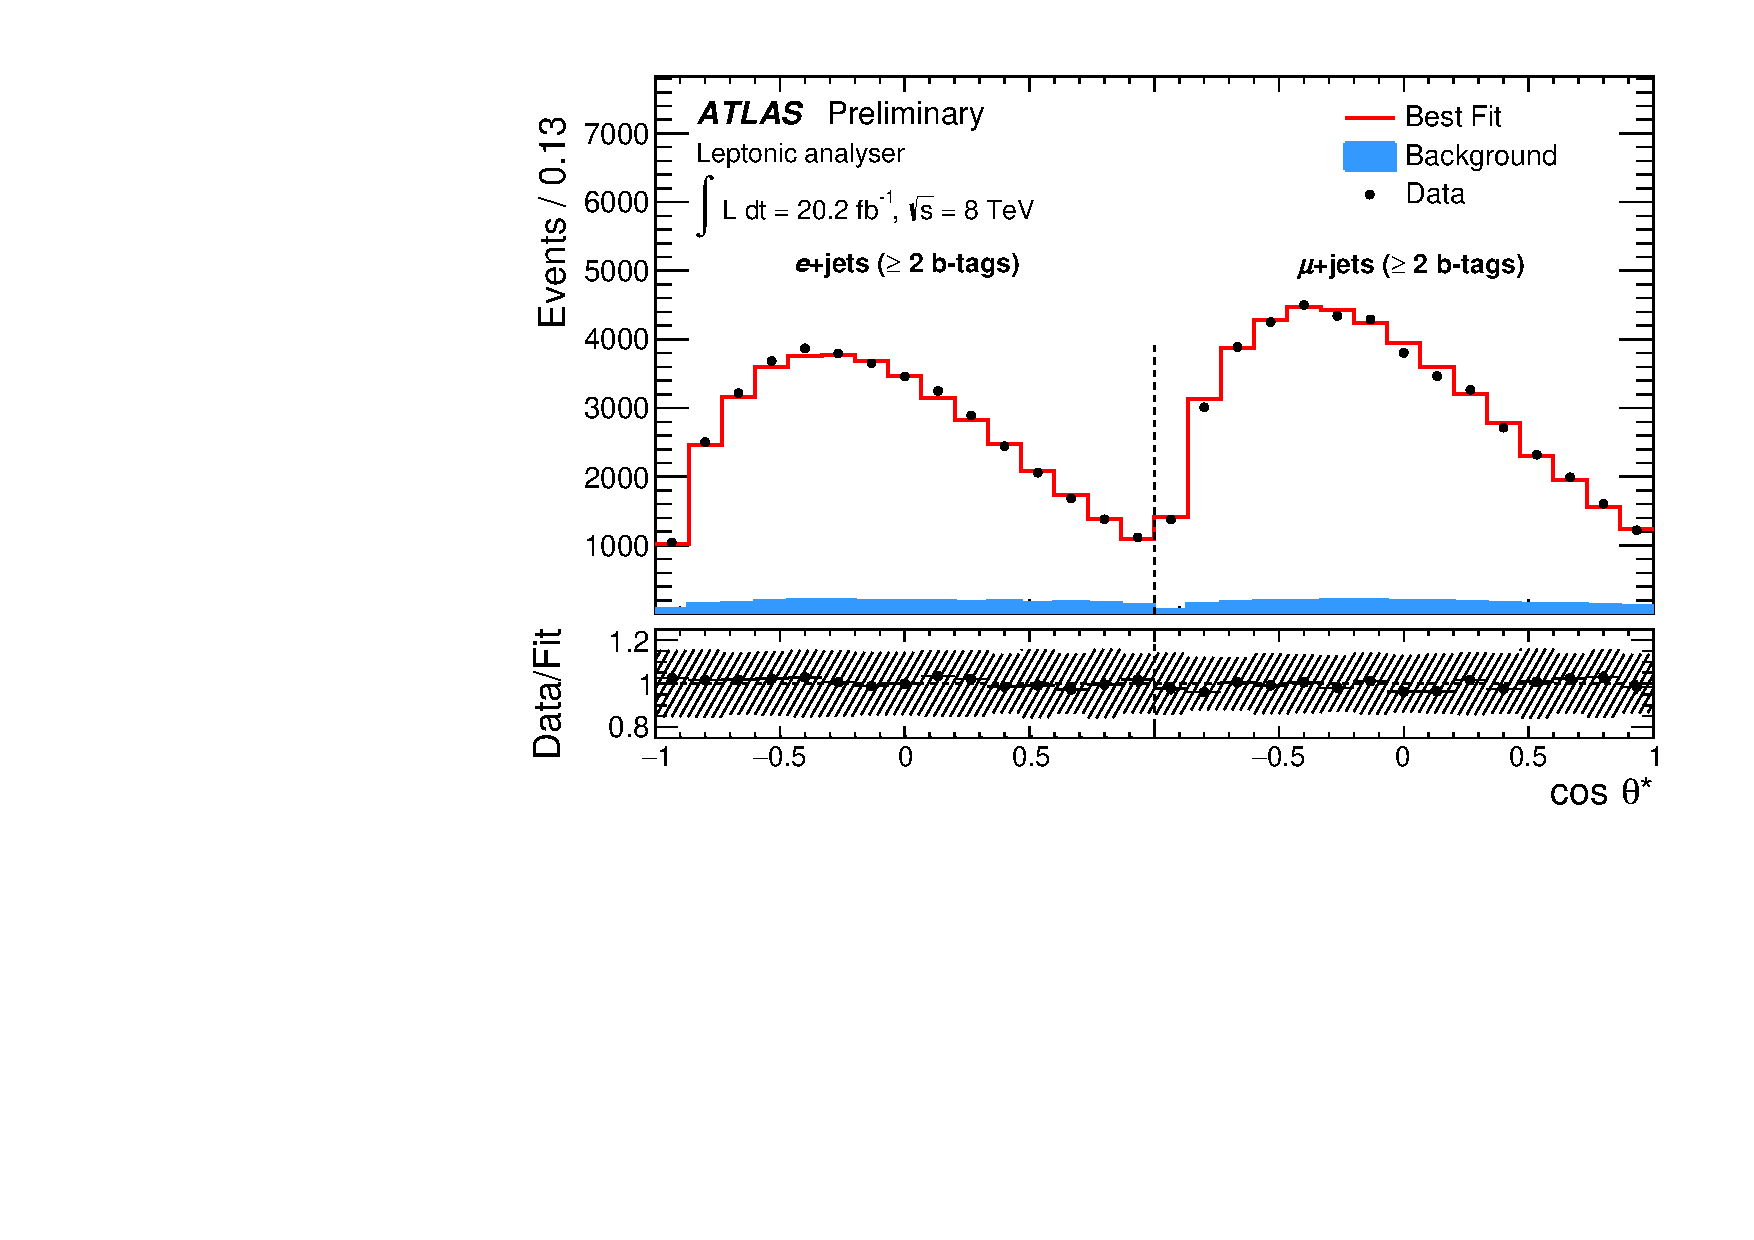
\includegraphics[height=70mm]{chapters/whel/figures/results/Datafit_StatUnc_el_mu_lep2incl}
		%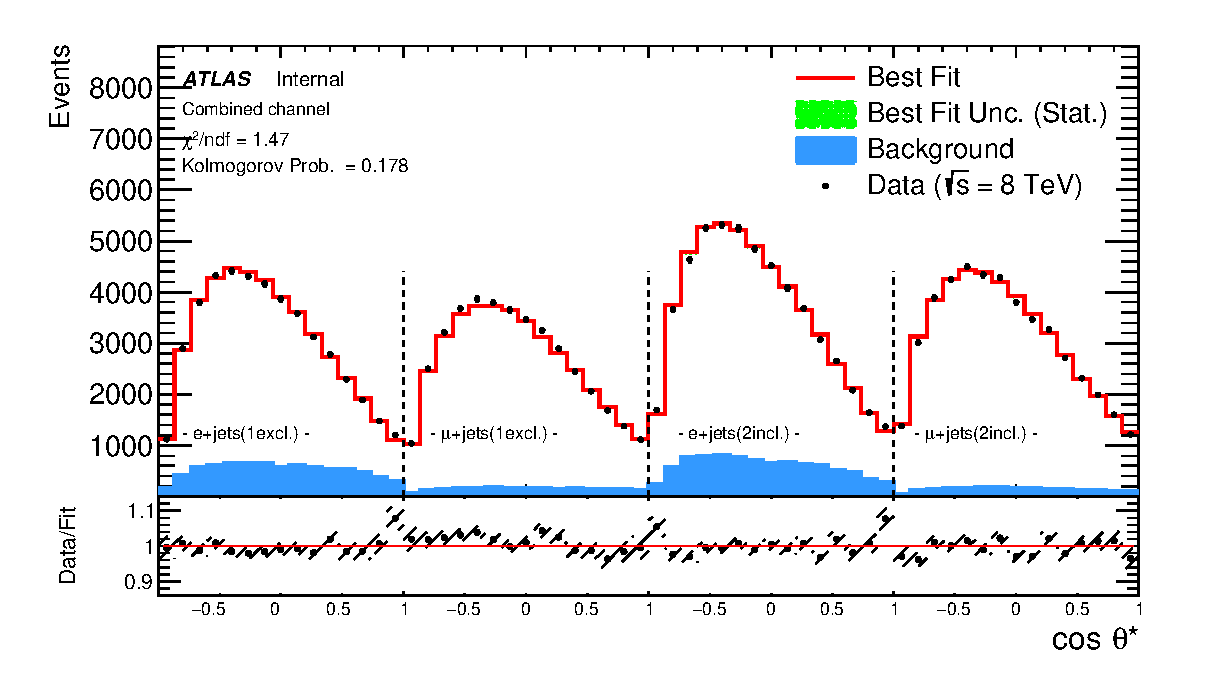
\includegraphics[height=70mm]{chapters/whel/figures/results/bTag_1excl2incl/Datafit_StatUnc_el_mu_bTag_lep}
		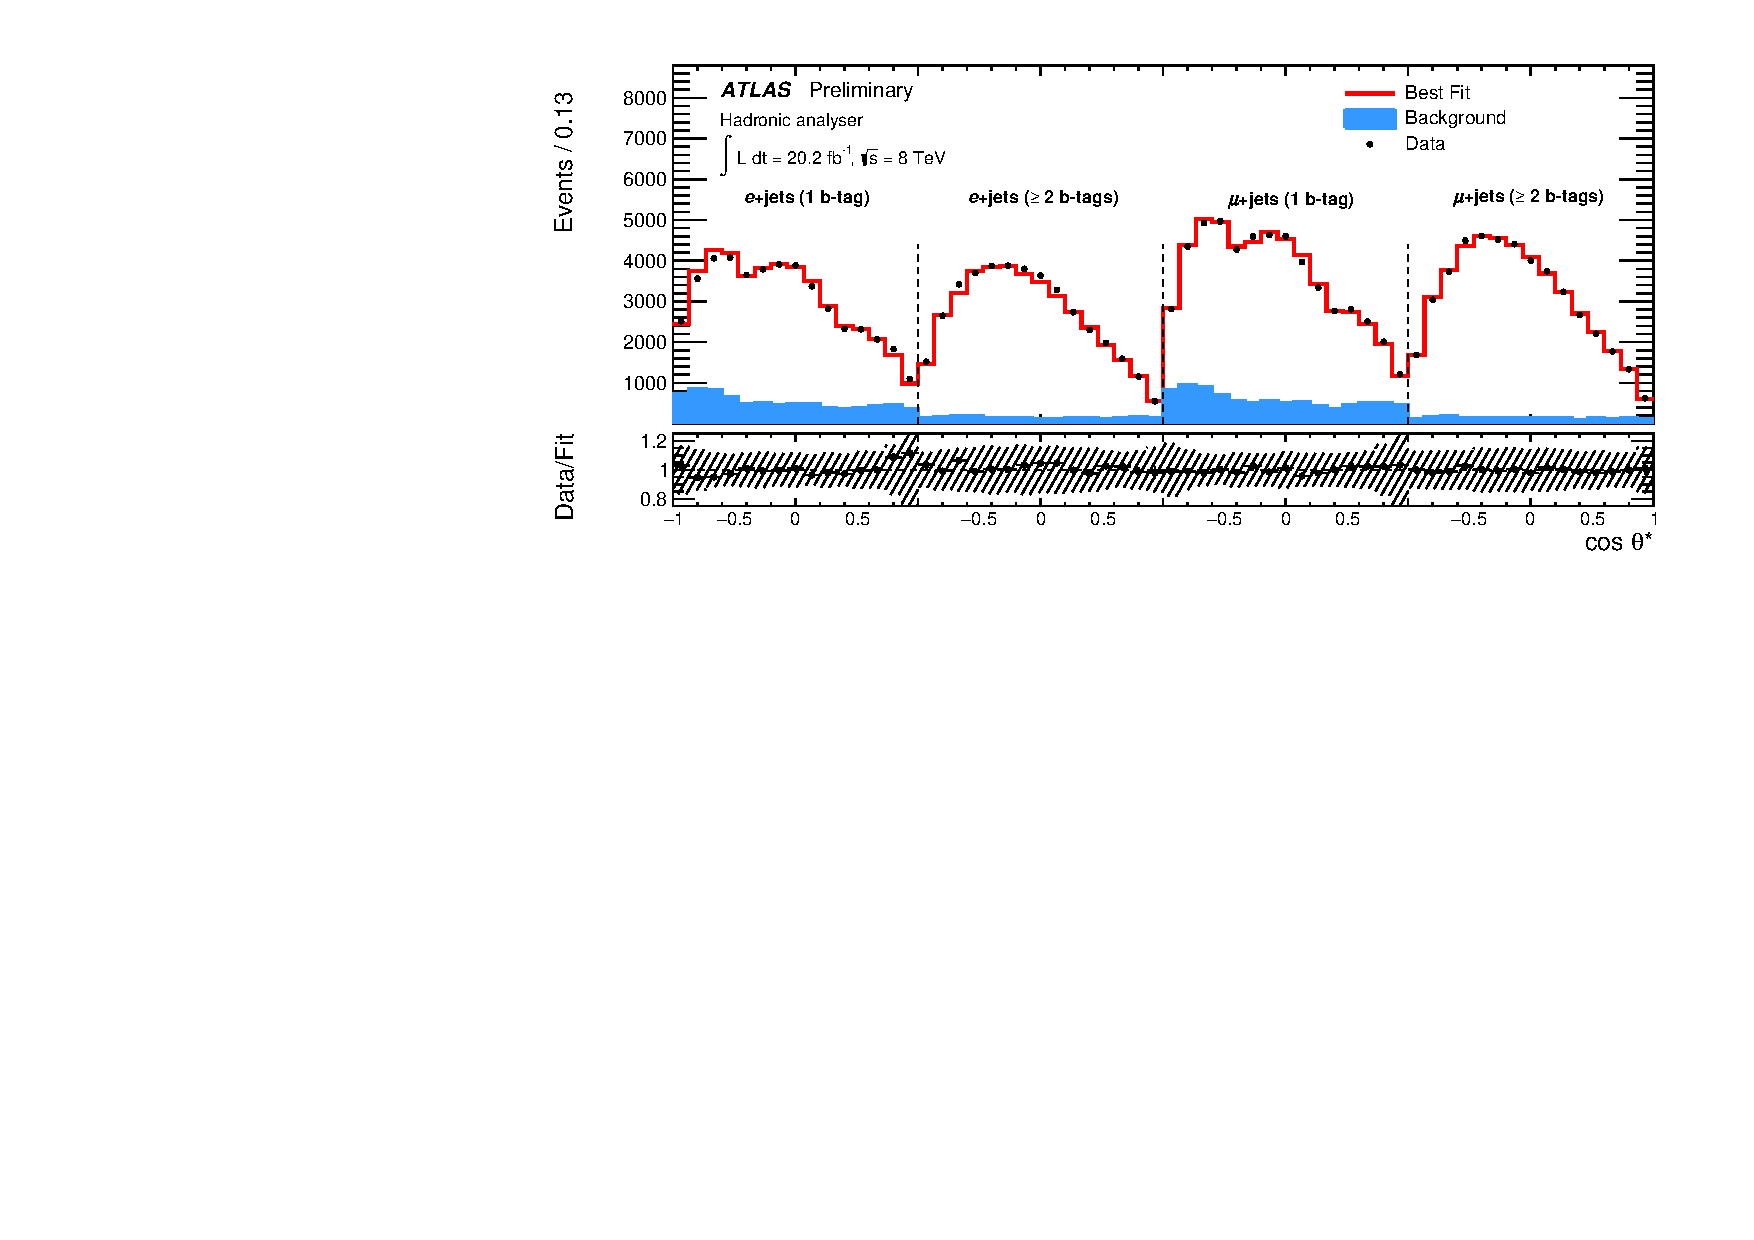
\includegraphics[height=70mm]{chapters/whel/figures/results/bTag_1excl2incl/Datafit_StatUnc_el_mu_bTag_had}
	%\caption{Fit results and statistical errors for the combined electron + muon channel in one exclusive + two inclusive \bt tag region for the leptonic angle (top) and the hadronic angle (bottom). Leptonic and hadronic measurements were fit separately.}
	\caption{Fit results and statistical + systematic errors for the combined electron + muon channel in two inclusive (one exclusive + two inclusive) \bt tag region for the leptonic (hadronic) analyzer at top (bottom).}
	%\label{fig:cosThetaFits_lep_and_had}
	\label{fig:cosThetaFits_lep_2incl_had_bTag}
\end{center}
\end{figure}

%\begin{figure}[!ht]
%\begin{center}
%		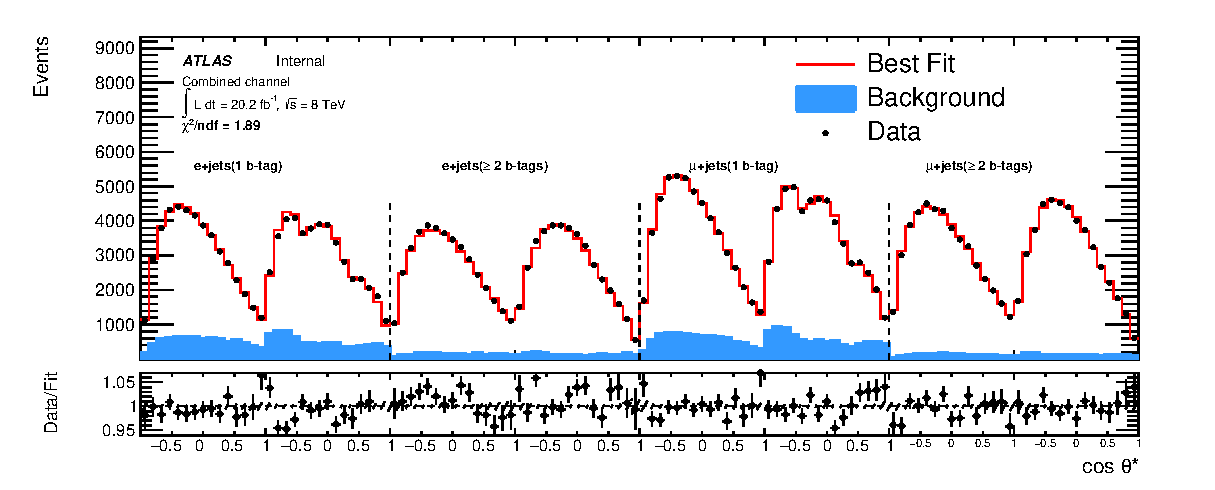
\includegraphics[height=70mm]{chapters/whel/figures/results/bTag_1excl2incl/Datafit_StatUnc_el_mu_lephad_bTag}
%	\caption{Fit results and statistical errors for the combined electron + muon channel in one exclusive + two inclusive \bt tag region for the leptonic + hadronic analyzers.}
%	\label{fig:cosThetaFits_lephad}
%\end{center}
%\end{figure}

%Two types of systematic uncertainties dominate: First, \bt-tagging is important in both the event selection and classification as well as in the dedicated up-/down-type separation. The other dominant contribution comes from the initial and final state radiation modeling. It influences jet properties (and hence object identification), modifies the misreconstruction due to combinatorial background and also directly influences the decay product kinematics.
The measured \w boson\ helicity fractions obtained using the leptonic branch of semileptonic \ttbar events with $\geq$2~$b$-tags are: 

%\begin{table}[h!]
\begin{center}
  \begin{tabular}{l}
\hline
%\hline
\multicolumn{1}{c}{Leptonic analyzer ($\geq$2 $b$-tags) }\\%[5pt]
\hline%\\%[1pt]
\fo = 0.709 $\pm$ 0.012 (stat.+bkg) ${}^{+0.015}_{-0.014}$ \syst     \\[5pt]
\fl = 0.299 $\pm$ 0.008 (stat.+bkg) ${}^{+0.013}_{-0.012}$ \syst    \\[5pt]
\fr = -0.008 $\pm$ 0.006 (stat.+bkg) $\pm 0.012$ \syst    \\[5pt]
\hline
%\hline
\end{tabular}
\end{center}
%\caption{Measured \w ~boson helicity fractions for the leptonic analyzer.}
%\label{tab:results_lep}
%\end{table}

By construction, the individual fractions sum up to one. The \fo value is anti-correlated with both \fl and \fr ($\rho_{F_0, F_L}$=~-0.55, $\rho_{F_0, F_R}$=~-0.75), and \fl and \fr are positively correlated ($\rho_{F_L, F_R}$=~+0.16). The quoted values correspond to the total correlation coefficient, considering both statistical and systematic uncertainties. These results are the most accurate \w boson\ helicity fractions measured to date and are consistent with the SM predictions given at NNLO accuracy~\cite{nnlo_theory}.

The most sensitive \w boson\ helicity fractions obtained using the hadronic analyzer are measured using the combination of events with 1~\bt tag and $\geq$~2\bt-tags. The results are given in Table~\ref{tab:other_results}. In the hadronic analyzer, the lower separation between the three \w boson\ helicity fraction signal templates results in smaller degree of correlations but larger systematic uncertainties. Combining the leptonic and hadronic analyzers is found to improve the statistical error and several sources of systematic error, but the the total systematic uncertainty is found to be larger than that estimated in the leptonic, two inclusive \bt tag measurement. The individual leptonic and hadronic measurements do however yield consistent results in agreement with each other.
%This should be a discussion some of the items in the table. For instance, this would be a good place to draw attention to the fact that radiation is probably by far the largest contribution to the systematic uncertainty. Following that, JER is probably the sub-leading. The two of these make up $\sim70-80\%$ of the total uncertainty. Looking at these two sources alone, we can see the improvement gained from the full combination across all regions. As described in Section \ref{sec:templateFitting}, the most sensitive final results are obtained from the eight-channel combination. Additionally, it is clear that some other sources of uncertainty probably don't play a very large role, and this is probably really cool.

%The final results for the leptonic helicity fractions in the combined electron + muon, 1 exclusive + 2 inclusive \bt tag region are \fo$= 0.XXX \pm 0.XXX$ \stat $\pm 0.XXXX$ \syst, \fl$= 0.XXX \pm 0.XXX$ \stat $\pm 0.XXXX$ \syst, \fr$= 0.XXX \pm 0.XXX$ \stat $\pm 0.XXXX$ \syst. The corresponding hadronic measurements in the combined lepton, combined \bt tag region are \fo$= 0.XXX \pm 0.XXX$ \stat $\pm 0.XXXX$ \syst, \fl$= 0.XXX \pm 0.XXX$ \stat $\pm 0.XXXX$ \syst, \fr$= 0.XXX \pm 0.XXX$ \stat $\pm 0.XXXX$ \syst.
%The final combination of the leptonic and hadronic measurements (eight-channel combination) yields results of  \fo$= 0.674 \pm 0.007$ \stat $\pm$0.027 \syst, \fl$= 0.315 \pm 0.005$ \stat $\pm 0.016$ \syst, \fr$= 0.011 \pm 0.004$ \stat $\pm 0.028$ \syst. The final measurement in the leptonic, two inclusive \bt tag region yields results of  \fo$= 0.709 \pm 0.012$ \stat $\pm$0.022 \syst, \fl$= 0.299 \pm 0.008$ \stat $\pm 0.011$ \syst, \fr$= -0.008 \pm 0.006$ \stat $\pm 0.019$ \syst.

In the case of the leptonic analyzer, the dominant systematic uncertainty contributions come from jet energy scale and resolution and the limited statistics in the MC templates. The systematic uncertainties in the hadronic measurement are smaller in the one exclusive plus two inclusive \bt tag region compared to the two inclusive tag region alone. Adding the one exclusive region to the leptonic analyzer is not found to improve sensitivity compared to the two inclusive region measurement. The largest systematic contribution comes from the \bt tagging uncertainty which affects the event selection, the \bt tag classification, and the up- vs. down-type quark separation. Other major contributions come from jet energy resolution, the modeling of \ttbar\ events (initial and final state radiation, parton showering and hadronization, and Monte Carlo generator choice for the matrix elements), all of which directly affect the object kinematics.

\begin{table}[h!]                                                                                                                                
  \centering
  \begin{tabular}{l}
\hline \hline
\multicolumn{1}{c}{Leptonic, 2 Incl., $e+\mu$ Combination}\\
\hline
\fo = 0.709  $\pm$ 0.012 (stat.+bkg) $\pm$ 0.015 \syst     \\
\fl = 0.299  $\pm$ 0.008 (stat.+bkg) $\pm$ 0.014 \syst    \\
\fr = -0.008 $\pm$ 0.006 (stat.+bkg) $\pm$ 0.012 \syst    \\ \hline \hline
\multicolumn{1}{c}{Lep + Had, 2 Incl., $e+\mu$ Combination}\\
\hline
\fo = 0.694  $\pm$ 0.009 (stat.+bkg) $\pm$ 0.029 \syst     \\
\fl = 0.308  $\pm$ 0.006 (stat.+bkg) $\pm$ 0.019 \syst    \\
\fr = -0.002 $\pm$ 0.005 (stat.+bkg) $\pm$ 0.016 \syst    \\ \hline \hline
\multicolumn{1}{c}{Leptonic, 1 Excl. + 2 Incl., $e+\mu$ Combination}\\
\hline
\fo = 0.686 $\pm$ 0.010 (stat.+bkg) $\pm$ 0.043 \syst     \\
\fl = 0.308 $\pm$ 0.006 (stat.+bkg) $\pm$ 0.015 \syst    \\
\fr = 0.006 $\pm$ 0.005 (stat.+bkg) $\pm$ 0.035 \syst    \\ \hline \hline

\multicolumn{1}{c}{Hadronic, 1 Excl. + 2 Incl., $e+\mu$ Combination}\\
\hline
\fo = 0.659 $\pm$ 0.010 (stat.+bkg) $\pm$ 0.054 \syst     \\
\fl = 0.281 $\pm$ 0.021 (stat.+bkg) $\pm$ 0.067 \syst    \\
\fr = 0.061 $\pm$ 0.022 (stat.+bkg) $\pm$ 0.108 \syst   \\ \hline \hline

\multicolumn{1}{c}{Lep + Had, 1 Excl. + 2 Incl., $e+\mu$ Combination}\\
\hline
\fo = 0.674 $\pm$ 0.007 (stat.+bkg) $\pm$ 0.027 \syst     \\
\fl = 0.315 $\pm$ 0.005 (stat.+bkg) $\pm$ 0.016 \syst    \\
\fr = 0.011 $\pm$ 0.004 (stat.+bkg) $\pm$ 0.023 \syst    \\ \hline \hline
\end{tabular}
\caption{Obtained \w helicity fractions in different sorts of combination w.r.t the \bt tag, analyzer and lepton channels.}
\label{tab:other_results}
\end{table}


%The overall error is worse in the total combination is worse than the combination in the two inclusive \bt tag region due to the increased impact of the systematic errors in the one exclusive \bt tag region. The two inclusive combination provides the best overall result and so is quoted as the final result in the hadronic channel. 

%This analysis represents the first measurement of the \w boson polarization fractions using a dedicated up and down type quark separation for the hadronic analyzer. Compared to the leptonic, one exclusive + two inclusive \bt tag region, the addition of the hadronic measurement improves the sensitivity in the measurement of the left-handed fraction. While the fully combined results (leptonic + hadronic, one exclusive + two inclusive \bt tag) have the smallest statisical error, the most precise determination of the \w boson polarization fractions in semileptonic \ttbar\ events are measured using the leptonic, two inclusive \bt tag region. 

% All figures and tables should appear before the summary and conclusion.
% The package placeins provides the macro \FloatBarrier to achieve this.
% \FloatBarrier


\subsection{Constraints on $Wtb$ Vertex}
%The final fitted helicity fractions can be used to constrain anomalous couplings in related to the production of \ttbar. Any deviation of \fo , \fl , \fr (or $A_{+}$ and $A_{-}$ ) from the Standard Model prediction could be caused by new physics contributing to the \Wtb vertex, and so the final fitted helicity fractions can be used to constrain any such anomalous couplings/new interactions associated with the top quark may exist at higher energies. The \Wtb vertex can be parameterized in terms of an effective Lagrangian~\cite{JAASandCia_ProbingWtb} above the electroweak symmetry breaking scale of $v = 246$ GeV. After electroweak symmetry breaking, this effective Lagrangian can be written as
The final fitted helicity fractions can be used to constrain anomalous couplings related to the production of \ttbar. Any deviation of \fo , \fl , \fr from the Standard Model prediction could be caused by new physics contributing to the \Wtb vertex, and so the final fitted helicity fractions can be used to constrain any such anomalous couplings/new interactions associated with the top quark may exist at higher energies. The \Wtb vertex can be parameterized in terms of an effective Lagrangian~\cite{JAASandCia_ProbingWtb} above the electroweak symmetry breaking scale of $v = 246$ GeV. After electroweak symmetry breaking, this effective Lagrangian can be written as

\begin{equation}
\mathscr{L}_{Wtb}= - \frac{g}{\sqrt{2}}\bar{b}\gamma^{\mu}(V_{L}P_{L}+ V_{R}P_{R}) t W_{\mu}^{-} - \frac{g}{\sqrt{2}}\bar{b}\frac{i\sigma^{\mu \nu}q_{\nu}}{M_{W}}(g_{L}P_{L}+ g_{R}P_{R}) t W_{\mu}^{-} + h.c.
\label{eq:lag}
\end{equation}

where $P_{\text{L}}$ ($P_{\text{R}}$) is the left-handed (right-handed) chirality operator and 

\begin{equation}
V_{L}= V_{tb}+C_{\phi q}^{(3,3+3)}\frac{\nu^{2}}{\Lambda^{2}},  V_{R}= \frac{1}2 C_{\phi \phi^{*}}^{(33)}\frac{\nu^{2}}{\Lambda^{2}},  g_{L}= \sqrt{2}C_{dW^{*}}^{(33)}\frac{\nu^{2}}{\Lambda^{2}},  ~g_{R}= \sqrt{2}C_{uW}^{(33)}\frac{\nu^{2}}{\Lambda^{2}},
\end{equation}

The parameter $\Lambda$ is the new physics scale and $C_{\phi q}^{(3,3+3)}$, $C_{\phi\phi^*}^{(33)}$, $C_{dW^{*}}^{(33)}$, and $C_{uW}^{(33)}$ are the effective operator coefficients. The anomalous couplings $V_{\text{R}}$, $g_{\text{L}}$, and $g_{\text{R}}$, generated by dimension-six operators, are absent in the Standard Model at tree level while the coupling $V_{tb}$ receives a correction from the operator $C_{\phi q}^{(3,3+3)}$. The effect of non-vanishing $V_{\text{R}}$, $g_{\text{L}}$, and $g_{\text{R}}$ on the observables $F_{i}$ has been calculated in \cite{anom1,anom2}. As an example, Figure \ref{fig:anom_fl} shows the influence on \fl~\cite{eftfitter}.

\begin{figure}[!ht]
\begin{center}

		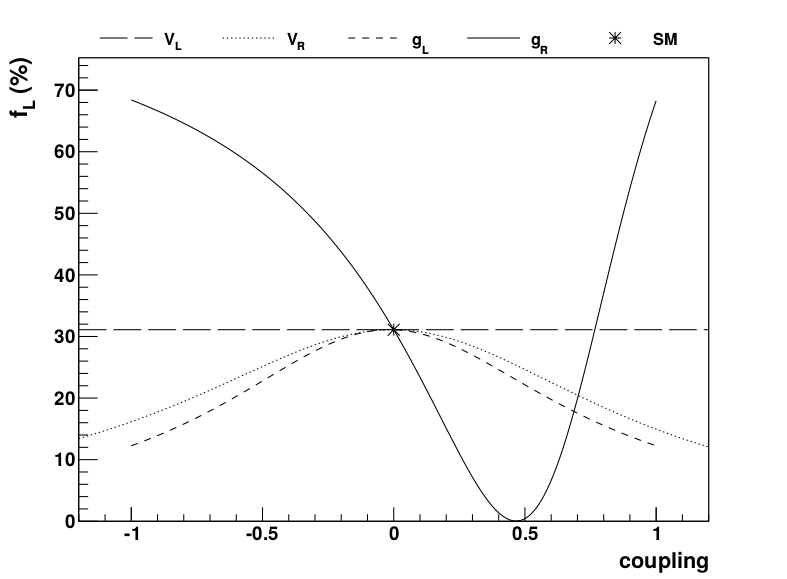
\includegraphics[height=62mm]{chapters/whel/figures/anomalousWtb/FL.png}
	\caption{Effect of modified anomalous couplings $V_{\text{R}}$, $g_{\text{L}}$, and $g_{\text{R}}$ on the fraction of longitudinally polarized $W$ bosons as implemented in EFTfitter. For each coupling, the value is varied over [-1, 1] (x-axis) while the others are held fixed to their SM values.}
	\label{fig:anom_fl}
\end{center}
\end{figure}

Limits on anomalous couplings ($V_{\text{R}}$, $g_{\text{L}}$, and $g_{\text{R}}$) are obtained from the measurement of the \w boson helicity fractions in two inclusive \bt tag region of the leptonic analyzer by utilizing the dependence of the fractions on the couplings. The \texttt{EFTfitter} tool \cite{eftfitter} is used to extract limits on the anomalous couplings. For simplicity, all couplings are assumed to be real. The limit setting makes use of the measured helicity fractions \fo\ and \fl\ as well as their total uncertainties. The third fraction, \fr, is considered via the constraint of $\sum F_i = 1$. As the correct correlation between the uncertainties is crucial for the limit setting, the total covariance matrix was derived and provided as input for \texttt{EFTfitter}. 
%As the correct correlation between the uncertainties is crucial for the limit setting, the total covariance matrix was derived (see Appendix \ref{app:covMatrix}) and provided as input for \texttt{EFTfitter}. 

Results showing the 68\% and 95.5\% posterior integrals for $g_{\text{L}}$ and $g_{\text{R}}$ (while fixing $V_L = 1$, $V_R = 0$) can be found in Figure~\ref{fig:anomalousLimits_2d_2ch}, as well as the 68\% and 95.5\% posterior integrals for $g_{\text{R}}$ and $V_{\text{R}}$, while fixing the other parameters to their SM values. %Figure \ref{fig:anomalousLimits_2d_2ch} shows the corresponding plots for the combination of the leptonic analyzer in the 2-$b$-tag incl. channels. 

In Figure \ref{fig:anomalousLimits_1d_2ch}, the one-dimensional limits for each anomalous coupling are shown (for all other couplings fixed to their SM expectation). %Figure \ref{fig:anomalousLimits_1d_2ch} shows the corresponding plots for the combination of the leptonic analyzer in the 2 $b$-tag incl. channels.
The  95.5\% CL intervals for the anomalous couplings are also summarized in Table \ref{tab:1d_limits_2ch}. %for the full combination and in Table \ref{tab:1d_limits_2ch} for the combination of the leptonic analyzer in the 2-$b$-tag incl. channels.

%\begin{table}[h!]                                                                                                                                
%  \centering
%  \begin{tabular}{l | l}
%Coupling & 95\,\% CL limit\\
%\hline
%\hline
%  $V_{\text{R}}$ & $[-0.xxx, 0.xxx]$\\
%  $g_{\text{L}}$ & $[-0.xxx, 0.xxx]$\\
%   $g_{\text{R}}$ & $[-0.xxx, 0.xxx], [0.xxx, 0.xxx]$\\
%\end{tabular}
%\caption{Limits for the anomalous coulings $V_{\text{R}}$, $g_{\text{L}}$, and $g_{\text{R}}$ at 95.5\,\% CL. The limtis were derived using the measured \Wboson\ helicity fractions (combination of all eight channels).}
%\label{tab:1d_limits}
%\end{table}

\begin{table}[h!]                                                                                                                                
  \centering
  \begin{tabular}{l | l}
Coupling & 95.5\% CL limit\\
\hline
\hline
  $V_{\text{R}}$ & $[-0.24, 0.31]$\\
  $g_{\text{L}}$ & $[-0.14, 0.11]$\\
   $g_{\text{R}}$ & $[-0.02, 0.06], [0.74, 0.78]$\\
\end{tabular}
\caption{Limits for the anomalous couplings $V_{\text{R}}$, $g_{\text{L}}$, and $g_{\text{R}}$ at 95.5\,\% CL. The limits were derived using the measured \Wboson\ helicity fractions (combination of the two channels using the leptonic analyzer in the 2-$b$-tag incl. channels).}
\label{tab:1d_limits_2ch}
\end{table}

%%


%\begin{figure}[!hb]
%\begin{center}

%		\includegraphics[width=0.45\textwidth]{figures/anomalousWtb/new_8channel/glgr}
%				\includegraphics[width=0.45\textwidth]{figures/anomalousWtb/new_8channel/vrgr}
%	\caption{\textcolor{red}{To be updated or removed} Left: Allowed regions at 68\%, 95.5\% and 99.7 \% confidence level (CL) for the \Wtb anomalous couplings $g_{\text{L}}$ and $g_{\text{R}}$. The other couplings are fixed to their SM expectation ($V_L = 1$, $V_R = 0$). Right: Corresponding limits on $V_{\text{R}}$ and $g_{\text{R}}$ for the other couplings fixed to their SM expectation. The limits were obtained using the 8-channel combination.}
%	\label{fig:anomalousLimits_2d}
%\end{center}
%\end{figure}

%\begin{figure}[!hb]
%\begin{center}
%		\includegraphics[height=62mm]{figures/anomalousWtb/new_8channel/gL} \\
%		\includegraphics[height=62mm]{figures/anomalousWtb/new_8channel/gR}
%		\includegraphics[height=62mm]{figures/anomalousWtb/new_8channel/VR} \\
%	\caption{\textcolor{red}{To be updated or removed} Limits on $V_R$, $g_{\text{L}}$ and $g_{\text{R}}$ while fixing the other anomalous couplings to their SM values. The limits were obtained using the 8-channel combination.}
%	\label{fig:anomalousLimits_1d}
%\end{center}
%\end{figure}

%%
\begin{figure}[!h]
\begin{center}

		\includegraphics[width=0.45\textwidth]{chapters/whel/figures/anomalousWtb/new_lep2incl/glgr}
				\includegraphics[width=0.45\textwidth]{chapters/whel/figures/anomalousWtb/new_lep2incl/vrgr}
	\caption{Left: Allowed regions at 68\%, 95.5\% and 99.7 \% confidence level (CL) for the \Wtb anomalous couplings $g_{\text{L}}$ and $g_{\text{R}}$. The other couplings are fixed to their SM expectation ($V_L = 1$, $V_R = 0$). Right: Corresponding limits on $V_{\text{R}}$ and $g_{\text{R}}$ for the other couplings fixed to their SM expectation. The limits were obtained using the 2-channel combination (leptonic analyzer, 2 b-jet incl.).}
	\label{fig:anomalousLimits_2d_2ch}
\end{center}
\end{figure}

\begin{figure}[!h]
\begin{center}
		\includegraphics[height=62mm]{chapters/whel/figures/anomalousWtb/new_lep2incl/gL} \\
		\includegraphics[height=62mm]{chapters/whel/figures/anomalousWtb/new_lep2incl/gR}
		\includegraphics[height=62mm]{chapters/whel/figures/anomalousWtb/new_lep2incl/VR} \\
	\caption{Limits on $V_R$, $g_{\text{L}}$ and $g_{\text{R}}$ while fixing the other anomalous couplings to their SM values. The limits were obtained using the 2-channel combination (leptonic analyzer, 2 b-jet incl). The arrows are drawn to explicitly show the value of the calculated global mode for each coupling.}
	\label{fig:anomalousLimits_1d_2ch}
\end{center}
\end{figure}

The results are in good agreement with the SM expectations.
